\section{Tornado Cash Heuristics}
\label{sec:tornado}

Focusing on the subset of Ethereum transaction data involving Tornado cash deposits and withdrawals, we discuss a collection of heuristics for identifying compromised deposits.

\subsection{Address Match}

\begin{figure}[h!]
\centering
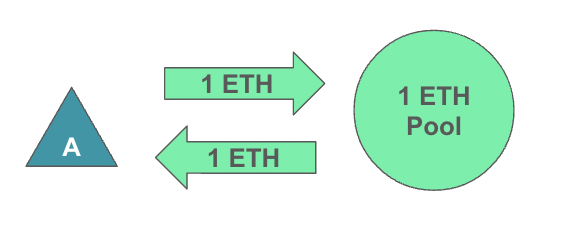
\includegraphics[width=0.75\linewidth]{figures/tcash/h1.png}
\caption{Address match -- The triangle represents a single address withdrawing and depositing to a TC pool.}
\label{fig:tornado}
\end{figure}

Suppose the address making a deposit transaction to a Tornado Cash pool matches the address making a withdrawal transaction (from the same pool). In that case, the two transactions can be linked, and the corresponding deposit is compromised as the user identity may be revealed. These may be TORN yield farmers who deposit and withdraw to the same address and are only profit-motivated or clumsy Tornado cash users.

\subsection{Unique Gas Price}

\begin{figure}[h!]
\centering
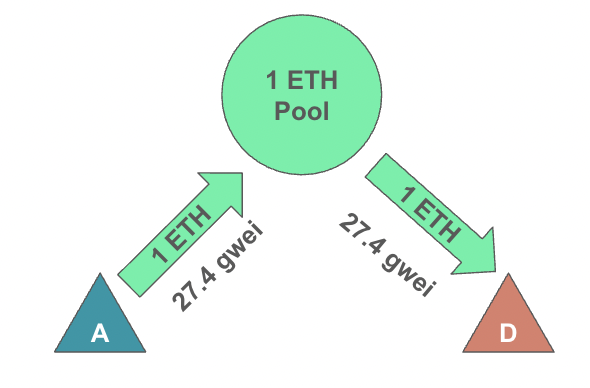
\includegraphics[width=0.7\linewidth]{figures/tcash/h2.png}
\caption{Unique gas price -- two addresses depositing and withdrawing with the same 27.4 gwei gas price.}
\label{fig:tornado}
\end{figure}

Prior to EIP-1559, Ethereum users could specify the gas price when making a deposit or withdrawal to a Tornado Cash pool. Those who do so tend to specify gas prices that are identical for deposit and withdrawal transactions. User-specified gas prices follow common patterns such as being round numbers or being unique to an individual. Care must be taken to remove transactions made by a relayer service which may set gas prices as well. Relayer-specified prices tend to be oddly specific and not round numbers. In practice, relayers can be filtered out by decoding the input code from Ethereum transaction data.

\subsection{Linked ETH Addresses}

\begin{figure}[h!]
\centering
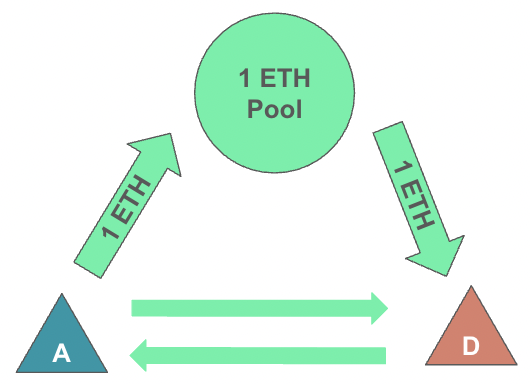
\includegraphics[width=0.6\linewidth]{figures/tcash/h3.png}
\caption{Linked ETH addresses -- the green arrows represent interactions between two addresses A and D outside of TC. Addresses A and D deposit and withdraw from the same TC pool, respectively.}
\label{fig:tornado}
\end{figure}

This heuristic aims to link withdraw and deposit transactions on Tornado Cash by inspecting ETH (non-Tornado Cash) interactions. This is done by constructing two sets, one corresponding to the unique Tornado Cash deposit addresses and one to the unique Tornado Cash withdraw addresses, to then make a query to reveal transactions between addresses of each set: when at least three such transactions are found, the withdraw and deposits addresses will be considered heuristically linked in Tornado Cash. The more transactions found, the more confident we are in the link.

\subsection{Multiple Denomination}

\begin{figure}[h!]
\centering
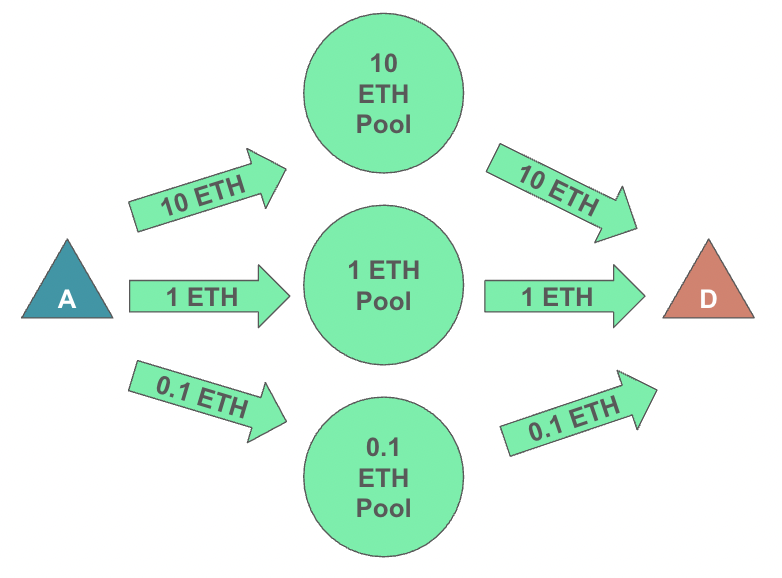
\includegraphics[width=0.6\linewidth]{figures/tcash/h4.png}
\caption{Multi Denomination -- Addresses A and D deposit and withdraw the same number of times from the same three TC pools, respectively.}
\label{fig:tornado}
\end{figure}

Previous heuristics examine isolated pairs of deposit and withdraw transactions. This heuristic, however, studies an address' history of transactions. We compute the portfolio of an address' withdraws across Tornado Cash pools, hence ``multi-denomination''. For instance, Alice may have withdrawn from the 1 ETH pool twice, the 0.1 ETH pool five times, the DAI pool once. Then we search for all addresses whose portfolio of deposit transactions is \textit{exactly the same} as Alice' withdrawal portfolio. An address withdrawing from the 1 ETH pool three times, the 0.1 ETH pool five times, and the DAI pool once would be a valid match. (Optionally, we can relax this to search for deposits with at least as many as Alice' withdraws, though this risks more false positives). All Tornado Cash transactions under the matched deposit and withdrawal address are linked to each other.

We ignore all addresses that make fewer than three transactions to Tornado Cash pools, and ignore all addresses that interact with only one pool. Additionally, to reduce the likelihood of false positives, we further constrain deposits within a multi-denomination reveal to occur within a 24 hour window; similarly we separately constrain withdraws within a multi-denomination reveal to occur within a 24 hour window. This intuition being that careless users will deposit or withdraw all at once.
% Unlike prior heuristics, this one has a higher chance of false positives. To address this, we assign a confidence to clustered transactions based on the difference in count between deposit and withdrawal portfolios. For an address $v$, we assign:
% \begin{equation*}
%   \kappa(v) = \frac{1}{\sum_{p \in \textup{pools}} |(\#D(v,p)) - (\#W(v,p))| }
% \end{equation*}
% where $\#D(v,p)$ is the number of deposit transactions made by address $v$ to pool $p$, and similarly $\#W(v, p)$ is the number of withdrawal transactions. We remove all transactions of addresses with confidence $\kappa(v) < 0.1$.

\subsection{TORN Mining}

\begin{figure}[h!]
\centering
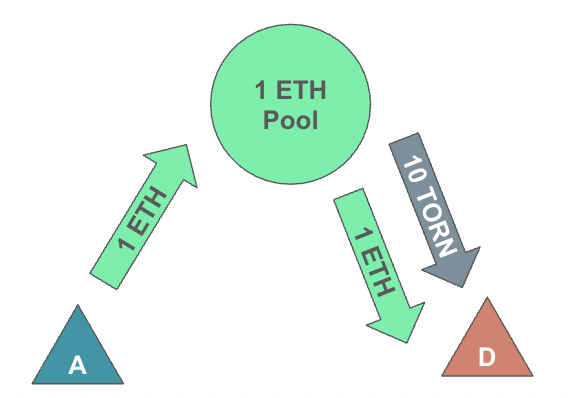
\includegraphics[width=0.6\linewidth]{figures/tcash/h5.png}
\caption{TORN Mining -- Address D was given 10 TORN upon withdrawing from the 1 ETH pool in return for anonymity points, linking address D to a deposit 100 blocks prior. Searching  records, only address A deposited in the 1 ETH pool 100 blocks prior, compromising address D. Note that the numbers presented here are for explanatory purposes.}
\label{fig:tornado}
\end{figure}

In February 2021, Tornado Cash introduced anonymity mining. It was an incentive scheme to encourage more deposits in Tornado Cash pools, thereby increasing their anonymity sets. Tornado Cash rewarded participants a fixed amount of anonymity points (AP) based on how long they left their assets in a pool.

After withdrawing assets, users can claim Anonymity Points. The amount withdrawn is recorded in the transaction. If a user uses a single address to claim all of their anonymity points, you can calculate the exact number of Ethereum blocks that their assets were in the pool because the AP yields were public and fixed. If there is a unique deposit / withdrawal combination in a pool separated by this number of Ethereum blocks, the transactions are assumed linked. This is more likely when the deposit or withdrawal in the pair also claimed the AP. This heuristic is most effective if AP is being claimed for a single deposit and is harder to compute for multiple deposits. 

\subsection{Connection to Tutela Clusters}

Unlike the Ethereum-wide heuristics (i.e., DAR and NODE), which find clusters of compromised \textit{addresses}, Tornado Cash heuristics find clusters of compromised \textit{transactions}. However, aside from address matching, a subset of these Tornado Cash heuristics can also be applied on the address level: given a cluster of compromised transactions, find the sender address for each transaction, and compute the unique set. Remove any addresses in our list of known addresses. These clusters can be added to the ones discussed in Section~\ref{sec:eth}.